\documentclass[a4paper,14pt]{extarticle}

% Путь до папки с общими шаблонами
\newcommand{\pathToCommonFolder}{../../Common}
% Название работы в титуле
\newcommand{\workname}{Отчет по практическим работам}
% Название дисциплины в титуле
\newcommand{\discipline}{Теория автоматов}
% Название кафедры в титуле
\newcommand{\kafedra}{Кафедра Вычислительной техники}
% Тема работы в титуле
\newcommand{\theme}{Сложение чисел с плавающей точкой}
% Должность преподавателя в титуле
\newcommand{\rang}{ассистент}
% ФИО преподавателя в титуле
\newcommand{\teacherfio}{А.~С.~Боронников}


\usepackage{tabularx}

\usepackage{booktabs}
\newcolumntype{b}{X}
\newcolumntype{s}{>{\hsize=.5\hsize}X}
\newcommand{\heading}[1]{\multicolumn{1}{c}{#1}}

\usepackage{extsizes} % Возможность сделать 14-й шрифт

% Вставка заготовки преамбулы
% Этот шаблон документа разработан в 2014 году
% Данилом Фёдоровых (danil@fedorovykh.ru) 
% для использования в курсе 
% <<Документы и презентации в \LaTeX>>, записанном НИУ ВШЭ
% для Coursera.org: http://coursera.org/course/latex .
% Исходная версия шаблона --- 
% https://www.writelatex.com/coursera/latex/5.3

% В этом документе преамбула

% Для корректного использования русских символов в формулах
% пакеты hyperref и настройки, связанные с ним, стоит загуржать
% перед загрузкой пакета mathtext



% поддержка русских букв
% кодировка шрифта
%\usepackage[T2A]{fontenc} 
\usepackage{pscyr}

% использование ненумеровонного абзаца с добавлением его в содержаниеl

\newcommand{\anonsection}[1]{\section*{#1}\addcontentsline{toc}{section}{#1}}
\newcommand{\sectionunderl}[1]{\section*{\underline{#1}}}


% настройка окружения enumerate
\usepackage{enumitem}
\setlist{noitemsep}
\setlist[enumerate]{labelsep=*, leftmargin=1.5pc}

\usepackage{hyperref}

% сначала ставить \usepackage{extsizes} % Возможность сделать 14-й шрифт
% для корректной установки полей вставлять преамбулу следует в последнюю очередь (но перед дерективой замены \rmdefault)
\usepackage[top=20mm,bottom=25mm,left=35mm,right=20mm]{geometry} % Простой способ задавать поля

\hypersetup{				% Гиперссылки
	unicode=true,           % русские буквы в раздела PDF
	pdftitle={Заголовок},   % Заголовок
	pdfauthor={Автор},      % Автор
	pdfsubject={Тема},      % Тема
	pdfcreator={Создатель}, % Создатель
	pdfproducer={Производитель}, % Производитель
	pdfkeywords={keyword1} {key2} {key3}, % Ключевые слова
	colorlinks=true,       	% false: ссылки в рамках; true: цветные ссылки
	linkcolor=red,          % внутренние ссылки
	citecolor=black,        % на библиографию
	filecolor=magenta,      % на файлы
	urlcolor=blue           % на URL
}

%%% Работа с русским языком
\usepackage{cmap}					% поиск в PDF
\usepackage{mathtext} 				% русские буквы в формулах
\usepackage[T2A]{fontenc}			% кодировка
\usepackage[utf8]{inputenc}			% кодировка исходного текста
\usepackage[english,russian]{babel}	% локализация и переносы
\usepackage{indentfirst}
\frenchspacing

%для изменения названия списка иллюстраций
\usepackage{tocloft}


\renewcommand{\epsilon}{\ensuremath{\varepsilon}}
\renewcommand{\phi}{\ensuremath{\varphi}}
\renewcommand{\kappa}{\ensuremath{\varkappa}}
\renewcommand{\le}{\ensuremath{\leqslant}}
\renewcommand{\leq}{\ensuremath{\leqslant}}
\renewcommand{\ge}{\ensuremath{\geqslant}}
\renewcommand{\geq}{\ensuremath{\geqslant}}
\renewcommand{\emptyset}{\varnothing}

% Изменения параметров списка иллюстраций
\renewcommand{\cftfigfont}{Рисунок } % добавляем везде "Рисунок" перед номером
\addto\captionsrussian{\renewcommand\listfigurename{Список иллюстративного материала}}

\newcommand{\tm}{\texttrademark\ }
\newcommand{\reg}{\textregistered\ }


%%% Дополнительная работа с математикой
\usepackage{amsmath,amsfonts,amssymb,amsthm,mathtools} % AMS
\usepackage{icomma} % "Умная" запятая: $0,2$ --- число, $0, 2$ --- перечисление

%% Номера формул
%\mathtoolsset{showonlyrefs=true} % Показывать номера только у тех формул, на которые есть \eqref{} в тексте.
%\usepackage{leqno} % Нумереация формул слева

%% Свои команды
\DeclareMathOperator{\sgn}{\mathop{sgn}}

%% Перенос знаков в формулах (по Львовскому)
\newcommand*{\hm}[1]{#1\nobreak\discretionary{}
{\hbox{$\mathsurround=0pt #1$}}{}}


% отступ для первого абзаца главы или параграфа
%\usepackage{indentfirst}

%%% Работа с картинками
\usepackage{graphicx}  % Для вставки рисунков
\graphicspath{{images/}{screnshots/}}  % папки с картинками
\DeclareGraphicsExtensions{.pdf,.png,.jpg}
\setlength\fboxsep{3pt} % Отступ рамки \fbox{} от рисунка
\setlength\fboxrule{1pt} % Толщина линий рамки \fbox{}
\usepackage{wrapfig} % Обтекание рисунков текстом

%%% Работа с таблицами
\usepackage{array,tabularx,tabulary,booktabs} % Дополнительная работа с таблицами
\usepackage{longtable}  % Длинные таблицы
\usepackage{multirow} % Слияние строк в таблице

%%% Теоремы
\theoremstyle{plain} % Это стиль по умолчанию, его можно не переопределять.
\newtheorem{theorem}{Теорема}[section]
\newtheorem{proposition}[theorem]{Утверждение}

\theoremstyle{plain} % Это стиль по умолчанию, его можно не переопределять.
\newtheorem{work}{Практическая работа}[part]


 
 
\theoremstyle{definition} % "Определение"
\newtheorem{corollary}{Следствие}[theorem]
\newtheorem{problem}{Задача}[section]
 
\theoremstyle{remark} % "Примечание"
\newtheorem*{nonum}{Решение}



%%% Программирование
\usepackage{etoolbox} % логические операторы

%%% Страница

%	\usepackage{fancyhdr} % Колонтитулы
% 	\pagestyle{fancy}
%   \renewcommand{\headrulewidth}{0pt}  % Толщина линейки, отчеркивающей верхний колонтитул
% 	\lfoot{Нижний левый}
% 	\rfoot{Нижний правый}
% 	\rhead{Верхний правый}
% 	\chead{Верхний в центре}
% 	\lhead{Верхний левый}
%	\cfoot{Нижний в центре} % По умолчанию здесь номер страницы

\usepackage{setspace} % Интерлиньяж
\onehalfspacing % Интерлиньяж 1.5
%\doublespacing % Интерлиньяж 2
%\singlespacing % Интерлиньяж 1

\usepackage{lastpage} % Узнать, сколько всего страниц в документе.

\usepackage{soul} % Модификаторы начертания


\usepackage[usenames,dvipsnames,svgnames,table,rgb]{xcolor}


\usepackage{csquotes} % Еще инструменты для ссылок

%\usepackage[style=authoryear,maxcitenames=2,backend=biber,sorting=nty]{biblatex}

\usepackage{multicol} % Несколько колонок

\usepackage{tikz} % Работа с графикой
\usepackage{pgfplots}
\usepackage{pgfplotstable}

% модуль для вставки рыбы
\usepackage{blindtext}

\usepackage{listings}
\usepackage{color}


% для поворота отдельной страницы. Использовать окружение \landscape
\usepackage{pdflscape} 
\usepackage{rotating} 


\definecolor{mygreen}{rgb}{0,0.6,0}
\definecolor{mygray}{rgb}{0.5,0.5,0.5}
\definecolor{mymauve}{rgb}{0.58,0,0.82}


% пример импорта файла
%\lstinputlisting{/home/denilai/repomy/conf/distributions}

\lstset{
	language=Python,
	basicstyle=\footnotesize,        % the size of the fonts that are used for the code
	numbers=left,                    % where to put the line-numbers; possible values are (none, left, right)
	numbersep=5pt,                   % how far the line-numbers are from the code
	numberstyle=\tiny\color{mygray}, % the style that is used for the line-numbers
	stepnumber=2,                    % the step between two line-numbers. If it's 1, each line will be numbered
	% Tab - 2 пробела
	tabsize=2,    
	% Автоматический перенос строк
	breaklines=true,
	frame=single,
	breakatwhitespace=true,
	title=\lstname 
}



% установка размера шрифта для всего документа
%\fontsize{20pt}{18pt}\selectfont


\author{Кирилл Денисов}
\title{Практическая работа №5}
\date{\today}

% установка полуторного интервала
% \usepackage{setspace}  
% \onehalfspacing

% использовать Times New Roman
\renewcommand{\rmdefault}{ftm}

\begin{document}
	
	\def\contentsname{ОГЛАВЛЕНИЕ}
	\setcounter{page}{3} % начать нумерацию с номера тр
	%\thispagestyle{empty}
	\tableofcontents
%	\listoffigures
%	\listoftables
%\thispagestyle{empty}


	
\begin{center}
	\newpage
%	\section*{Расчетно-пояснительная записка}
\end{center}
\section {Используемые сокращения}
%\begin{center}
ПЗ --- плавающая запятая

УА --- управляющий автомат

ОА --- операционный автомат

IEEE --- \textit{(англ. Institute of Electrical and Electronics Engineers)} институт инженеров электротехники и электроники

ПЗУ --- Постоянное запоминающее устройство \textit{(англ. ROM --- Read-only Memory)}

DI			---	Входная шина данных

 DO		---	Выходная шина данных
 
 OС		---	Код операции
 
 RI			---	Сигнал готовности данных
 
 RO		---	Выходной сигнал готовности
 

 
 OW		---	Сигнал переполнения разрядной сетки
 
 СOMP		---	компаратор
 
 CT			---	счетчик
 
 MX		---	мультиплексор
 
 RG		---	регистр
 
 
 SM		---	сумматор
%\end{center}
\section{Постановка задачи}
Разработать вычислительное устройство, состоящее из  двух взаимосвязанных частей --- операционного и управляющего автоматов, и выполняющее следующие операции:
\begin{enumerate}
	\item Деление двух целых чисел в дополнительном коде;
	\item Сложение чисел, представленных в экспоненциальном формате.
\end{enumerate}
Операнды представлены в виде 32-х двоичных разрядов. Управляющий автомат реализовать по схеме с регулярной адресацией в последовательном варианте.
\newpage
\section{Интерфейс устройства}
\label{sec:interface}
Приведем интерфейс разрабатываемого вычислительного устройства, обрабатывающий и формирующий на выходе 32-х разрядные числа (см. рис. \ref{fig:courseinterface}).
% TODO: \usepackage{graphicx} required
\begin{figure}[h!]
	\centering
	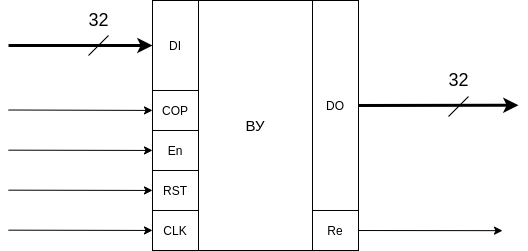
\includegraphics[width=0.7\linewidth]{images/course_interface}
	\caption{Интерфейс устройства}
	\label{fig:courseinterface}
\end{figure}
%\vspace{6em}
Представим устройство в виде композиции управляющего автомата (УА) и операционного автомата (ОА) --- рис. \ref{fig:courseinterfaceoama}.
% TODO: \usepackage{graphicx} required
\begin{figure}[h!]
	\centering
	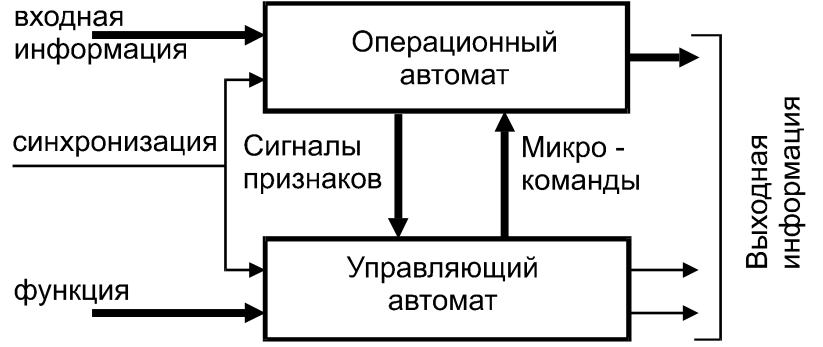
\includegraphics[width=0.7\linewidth]{images/course_interface_oa_ma}
	\caption{Композиция УА и ОА}
	\label{fig:courseinterfaceoama}
\end{figure}


\section{Формат данных}
 Данное вычислительное устройство оперирует с 32-х разрядными двоичными числами. От корректности их представления в конечном итоге зависит корректность производимых вычислений, поэтому соблюдение формата ввода/вывода критически важно при разработке вычислительного устройства. 
 
 Уточним принцип распознавания двоичных чисел, воспринимаемых вычислительным устройством.
 
 При выборе первой операции (деления двух целых чисел) будем использовать дополнительный код. Число будет представлено в виде 32-х разрядного двоичного числа.
 
 При выборе второй операции (сложения двух чисел) будем использовать стандарт IEEE 754, описывающий формат представления числе с плавающей точкой. Операнды представим в формате одинарной точности (\texttt{binary32}) (рис. \ref{fig:coursebinary32}). В этом формате под мантиссу числа отводится 24 разряда, а под экспоненту --- 8 разрядов. При чем один разряд отдан под знак. Смещение экспоненты в данном случае $2^7-1=127$. Минимальное и максимальное значение мантиссы, соответственно, $E_{min}=-126 E_{max}=127$.
 % TODO: \usepackage{graphicx} required
 \begin{figure}
 	\centering
 	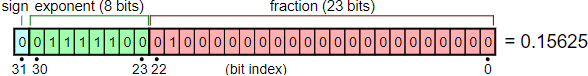
\includegraphics[width=0.7\linewidth]{images/course_binary32}
 	\caption{Число в формате одинарной точности}
 	\label{fig:coursebinary32}
 \end{figure}
 
 
\section{Назначение контактов}
Приведем назначение контактов разрабатываемого устройства согласно условному графическому обозначению интерфейса, приведенному в разделе \ref{sec:interface} (см. таблицы \ref{tab:inputs} и \ref{tab:outputs}).
\begin{table}[h!]
	\centering
	\begin{tabular}{|c|c|}
		\hline
		\multicolumn{1}{|c|}{\textbf{Вход}} & \multicolumn{1}{c|}{\textbf{Назначение}} \\ \hline
		DI & Входная 32-х разрядная шина данных \\ \hline
		OC & Код операции \\ \hline
		En & Разрешающий сигнал \\ \hline
		RST & Аппаратный сброс \\ \hline
		CLK & Синхронизирующий сигнал \\ \hline
	\end{tabular}
	\caption{Входы устройства}
	\label{tab:inputs}

\end{table}

\begin{table}[h!]
	\centering
	\begin{tabular}{|c|c|}
		\hline
		\multicolumn{1}{|c|}{\textbf{Выход}} & \multicolumn{1}{c|}{\textbf{Назначение}} \\ \hline
		DO & Выходная 32-х разрядная шина данных \\ \hline
		Re & Сигнал готовности результата \\ \hline
	\end{tabular}
	\caption{Выходы устройства}
	\label{tab:outputs}

\end{table} 


\section{Математическое обоснование алгоритмов}
\subsection{Деление двух целых чисел в дополнительном коде}
Для деления двух целых чисел представленных в двоичном дополнительном коде реализуем алгоритм деления без восстановления остатка. Данный способ деления, в отличие от алгоритма с восстановлением остатка, является оптимальным по суммарному времени, так как обработка очередного разряда результата осуществляется за один такт, ведь не нужно выполнять сложение для восстановления частичного остатка.

Опишем алгоритм деления следующим образом:
\begin{enumerate}
	\item \label{enum:first} Исходное значение частичного остатка полагается равным старшим разрядам делимого --- если делимое отрицательное, то все биты регистра частичного остатка устанавливаем в <<1>>, если делимое положительное, то все биты регистра частичного остатка устанавливаем в <<0>>;
	\item Частичный остаток удваивается путем сдвига на один разряд влево. При этом в освобождающийся при сдвиге младший разряд заносится очередная цифра делимого.
	\item Анализируем знаки остатка и делителя --- в случае, если их знаки одинаковые, то выполняем вычитание делителя из остатка (прибавляем противоположное число), полученного на данном этапе. Иначе же прибавляем значение делителя к значению остатка%
	\item \label{enum:last} Анализируем значение остатка после выполнения арифметических действий --- заносим в частное инвертированный знак остатка, вычисленного на данном этапе, вместе с этим сдвигая его влево. 
	\item Повторяем пункты \ref{enum:first}-\ref{enum:last} до тех пор, пока не будут сдвинуты все разряды делимого. 
\end{enumerate}

Стоит отметить, что для формирования правильного выходного результата после выполнения вышеперечисленных пунктов необходимо выполнить коррекцию значений частного и остатка в зависимости от знаков операндов. Для каждой комбинации знаков делимого и делителя реализована отдельная операция коррекции. См таблицу \ref{tab:correction4}.

\begin{table}[h!]
	\centering
	\begin{tabular}{|m{0.2\linewidth}|m{0.67\linewidth}|}
		\hline
		\textbf{Комбинация} &\multicolumn{1}{c|}{\textbf{Коррекция}}\\
		\hline
		$A\ge0, B>0 $ &Коррекция не требуется \\ 
		\hline
		$A\ge0, B<0$ & Изменить знак частного, остаток должен быть положительным\\
		\hline
		$A<0, B>0$ & Результат верен, если остаток $=0$. Иначе прибавить к отрицательному частному единицу. Остаток должен быть отрицательным\\
		\hline
		$A< 0, B< 0$ & Перед делением изменить знак делимого. Остаток должен быть отрицательными.\\
		\hline
	\end{tabular}
	\caption{Коррекция результата}
	\label{tab:correction4}
\end{table}
\subsection{Сложение чисел в экспоненциальной форме}
В арифметике с плавающей запятой сложение и вычитание — более сложные операции, чем умножение и деление. Обусловлено это необходимостью выравнивания порядков операндов. Алгоритм сложения и вычитания включает в себя следующие основные фазы:
\begin{enumerate}
	\item Определение операнда, имеющего меньший порядок, и сдвиг его мантиссы вправо на число разрядов, равное разности порядков операндов;
	\item Приравнивание порядка результата большему из порядков операндов;
	\item Сложение или вычитание мантисс и определение знака результата;
	\item Проверку па переполнение;
\end{enumerate}
C начала производится проверка с целью выяснения, не равен ли нулю один из операндов. Если это имеет место, в качестве результата сразу берется другой операнд.

В следующей фазе осуществляется выравнивание порядков обоих операндов. Для пояснения рассмотрим например сложения десятичных чисел с плавающей запятой: $123 \cdot 10^0 + 456 \cdot 10^{-2}$

Очевидно, что непосредственное сложение мантисс недопустимо, поскольку цифры мантисс, имеющие одинаковый вес, должны располагаться в эквивалентных позициях. Так, цифра 4 во втором числе должна суммироваться с цифрой 3 в первом. Этого можно добиться, если записать второе число так, чтобы порядки обоих чисел были равны:
\begin{align*}
123 \cdot 10^0 + 456 \cdot 10^{-2}= 123 \cdot 10^0 + 4,56 \cdot 10^0 = 127,56 х 10^0
\end{align*}

Выравнивания порядков можно достичь сдвигом мантиссы меньшего из чисел вправо, с одновременным увеличением порядка этого числа, либо сдвигом мантиссы большего из чисел влево и уменьшением его порядка. Оба варианта сопряжены с потерей цифр мантиссы, но выгоднее сдвигать \textit{меньшее} из чисел, так как при этом теряются младшие разряды мантиссы.

Таким образом, выравнивание порядков операндов реализуется путем сдвига мантиссы меньшего из чисел на один разряд вправо с одновременным увеличением порядка этого числа на единицу. Действия повторяются до совпадения порядков. Если в процессе сдвига мантисса обращается в 0,то в качестве результата операции берется другой операнд.

Следующая фаза --- сложение мантисс с учетом их знаков, что при одинаковых знаках мантисс может привести к переполнению. В последнем случае мантисса результата сдвигается вправо на один разряд, а порядок результата увеличивается на единицу. Это, в свою очередь, чревато переполнением поля порядка. Тогда операция прекращается и формируется \textit{признак переполнения}, сопровождаемый соответствующим предупреждением (обычно в виде сигнала прерывания).

В отличие от целочисленной арифметики, в операциях с ПЗ сложение и вычитание производятся приближенно, так как при выравнивании порядков происходит потеря младших разрядов одного из слагаемых. В этом случае погрешность всегда отрицательна и может доходить до единицы младшего разряда.
\if 0
Проектируя алгоритм вычислений будем исходить из следующих утверждений
\begin{itemize}
	\item Сумма дополнительных кодов чисел есть дополнительный код результата
	\item Сложение и вычитание производим в модифицированном дополнительном коде
	\item Признаком переполнения разрядной сетки сумматора дополнительного кода при сложении положительных чисел является отрицательный знак результата, а при сложении отрицательных чисел положительный знак результата
	\item Признаком нарушения нормализации числа справа ( когда величина результата равна или превышает единицу ) является наличие разноимённых комбинаций в знаковых разрядах сумматора
	\item  Признаком нарушения нормализации числа слева ( когда результат по абсолютной величине оказывается меньше 1/q ) является наличие одинаковых комбинаций в разряде переполнения и старшем разряде цифровой части сумматора
	\item Вычитание с плавающей точкой выполняем на сумматоре инвертировав знак мантиссы
\end{itemize}
\fi
При выполнении операции сложения предполагается, что числа, переданные на вход находятся в нормализованном виде, то есть имеют вид, представленный на сноске \ref{sign}.

\begin{equation}
\begin{aligned}
\label{sign}
\frac12&\le \left|M\right|< 1\\
M &= 0.1XXXX\\
M &= 1.0XXXX\\
M&=1.00000\\
\end{aligned}
\end{equation}

Результат суммы также нормализуется в соответствии с данными правилами. Числа, представленные в ином виде считаются ненормализованными и не обрабатываются цифровым устройством.

Стоит отметить, что для формирования правильного выходного результата необходимо выполнить нормализацию значений суммы в зависимости от вида операндов. Для каждой комбинации операндов реализована отдельная операция нормализации. См таблицу \ref{tab:correction5}.

\begin{table}[h!]
	\small
	\begin{tabular}{|m{0.2\linewidth}|m{0.73\linewidth}|}
		\hline
		\textbf{Комбинация} &\textbf{Коррекция}\\
		\hline
		$\left|m_a\pm m_b\right|\ge1$ & Мантисса не нормализована. Сдвинуть регистр мантиссы вправо, загрузить сигнал переноса сумматора. Увеличить порядок результата на 1. При этом может произойти переполнение счетчика в большую сторону \\ 
		\hline
		$\frac12\le \left|m_a\pm m_b\right|< 1$ & Нормализация результата не требуется\\
		\hline
		$\left|m_a\pm m_b\right|<\frac12$ & Мантисса не нормализована. Сдвигая мантиссу влево, уменьшать порядок, при этом может произойти переполнение порядка в отрицательную сторону\\
		\hline
	\end{tabular}
	\caption{Нормализация результата}
	\label{tab:correction5}
\end{table}



\section{Блок-схемы алгоритмов}
\subsection{Деление двух целых чисел в дополнительном коде}
Введем обозначения операндов, используемых в данной операции (таблица \ref{tab:vars}):
\begin{table}[h!]
	\small
	\centering
	\begin{tabular}{|c|c|}
		\hline
		\multicolumn{1}{|c|}{\textbf{Обозначение}} & \multicolumn{1}{c|}{\textbf{Назначение}} \\ \hline
		A & Делимое в доп. коде \\ \hline
		B & Делитель в доп. коде \\ \hline
		RES & Частное от деления \\ \hline
		REM & Остаток от деления \\ \hline
	\end{tabular}
	\caption{Операнды}
	\label{tab:vars}

\end{table} 

Опишем алгоритм выполнения деления  с помощью блок схемы.  См. рис.~\ref{img:algorithmcourse} в \hyperref[tam]{Приложении А}.


Теперь приведем блок-схему работу автомата, реализующий данный алгоритм, с указанием микрокоманд. См. рис. \ref{fig:coursealgorithmdividemachine} в \hyperref[tam]{Приложении А}. Используем счетчик для подсчета обработанных разрядов и регистры для хранения и использования разрядов делителя и делимого.
% TODO: \usepackage{graphicx} required


\subsection{Сложение чисел в экспоненциальной форме}
Опишем алгоритм выполнения суммы  с помощью блок схемы. См. рис.~\ref{fig:coursealgorithmsum}. в \hyperref[tam]{Приложении А}.
% TODO: \usepackage{graphicx} required

Теперь приведем блок-схему работу автомата, реализующий данный алгоритм, с указанием микрокоманд. См. рис. \ref{fig:coursealgorithmmachine2} в \hyperref[tam]{Приложении А}.

\section{Описание микрокоманд}
\subsection{Деление двух целых чисел в дополнительном коде}
Укажем необходимые признаки, которые впоследствии будут вырабатываться управляющим автоматом в ходе выполнения первой операции. См. таблицу \ref{tab:signalsop1}.
\begin{table}[h!]
	\small
	\centering
	\begin{tabular}{|m{0.2\linewidth}|m{0.7\linewidth}|}
		\hline
		\textbf{Признак} & \textbf{Назначение} \\ \hline
		$S$ & Хранит адрес следующей операции \\ \hline
		$Н$ & Адресный вход мультиплексора \\ \hline
		$R0$ & Сигнализирует об окончании операции деления \\ \hline
		$ERROR$ & Сигнализирует об ошибке ввода -- делитель равен нулю \\ \hline
		$L\_RG_A$ & Загрузка в регистр $RG\_A$ \\ \hline
		$L\_RG_B$ & Загрузка в регистр $RG\_B$ \\ \hline
		$L\_RG_REM$ & Загрузка в регистр $RG\_REM$ \\ \hline
		$CLR$ & Асинхронный сброс всех элементов \\ \hline
		$COUNT\_CT$ & Счет. Декремент счетчика, если $L\_CT==1$ \\ \hline
		$L\_CT$ & Загрузка счетчика \\ \hline
		$SHIFT$ & Левый сдвиг в регистрах $RG\_A \text{ и } RG\_RES$ \\ \hline
	\end{tabular}
	\caption{Деление чисел. Осведомительные сигналы (признаки)}
	\label{tab:signalsop1}
\end{table}

	

\subsection{Сложение чисел в экспоненциальной форме}

Укажем необходимые признаки, которые впоследствии будут вырабатываться управляющим автоматом в ходе выполнения второй операции. См. таблицу \ref{tab:signalsop2}.

\begin{table}[h!]
	\centering
	\small
	\begin{tabular}{|m{0.17\linewidth}|m{0.7\linewidth}|}
		\hline
		\textbf{Признак} & \textbf{Назначение} \\ \hline
		$S$ & Хранит адрес следующей операции \\ \hline
		$Н$ & Адресный вход мультиплексора \\ \hline
		$R0$ & Сигнализирует об окончании операции деления \\ \hline
		$overflow$ & Сигнализирует об ошибке обработки -- переполнение \\ \hline
		$L\_Ma$ & Загрузка в регистр $RG\_Ma$ \\ \hline
		$SHIFT\_Ma$ & Правый сдвиг регистра $RG\_Ma$ если $SHIFT\_Ma\_Left=0$ и левый, если  $SHIFT\_Ma\_Left=1$ \\ \hline
		$RST$ & Асинхронный сброс всех элементов \\ \hline
		$COUNT\_Pa$ & Счет. Декремент счетчика, если $L\_CT_\_Pa==1$ \\ \hline
		$L\_CT\_Pa$ & Загрузка счетчика $CT\_Pa$ \\ \hline
		$CHANGE$ & Выбор источника загрузки в регистры мантисс и порядка чисел A и B \\ \hline
		$e$ & Управляющий сигнал для счетчика. Если $e=1$, следует выполнить загрузку, а если $e=0$ -- инкрементировать счетчик. \\ \hline
	\end{tabular}
	\caption{Сложение чисел в экспоненциальной форме. Осведомительные сигналы (признаки)}
	\label{tab:signalsop2}
\end{table}
%\newpage




\section{Функциональная схема операционного автомата}
\subsection{Деление двух целых чисел в дополнительном коде}
Приведем функциональную схему операционного автомата, выполняющего деление двух целых чисел в дополнительном коде по алгоритму деления без восстановления остатков. См. рис. \ref{fig:courseoperationautomat}.

% TODO: \usepackage{graphicx} required
\begin{figure}[htp]
	\centering
	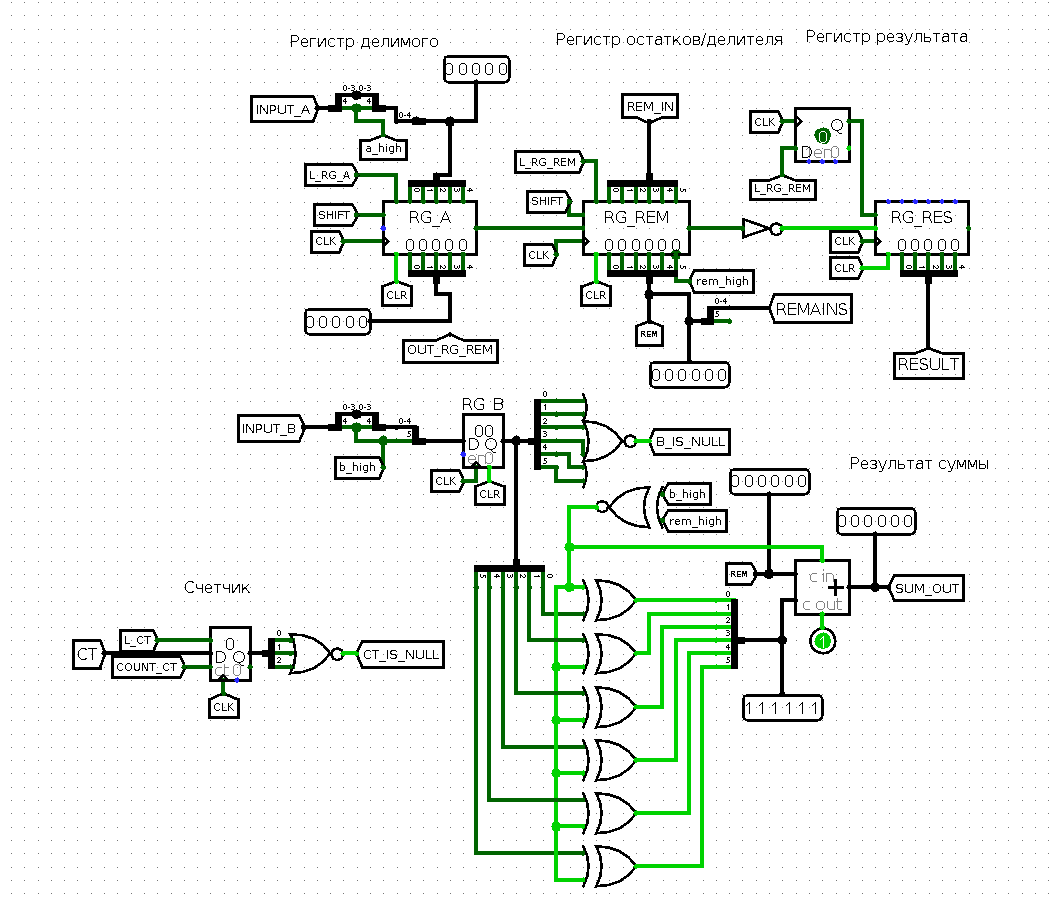
\includegraphics[width=0.8\linewidth]{images/course_operation_automat}
	\caption{Деление чисел. Операционный автомат}
	\label{fig:courseoperationautomat}
\end{figure}


Приведем названия и назначения каждого из регистров. См. таблицу \ref{tab:course_op1_regs}.
\begin{table}[h!]
	\centering
	\small
	\begin{tabular}{|m{0.2\linewidth}|m{0.6\linewidth}|}
		\hline
		\textbf{Идентификатор} & \textbf{Назначение} \\ \hline
		$RG\_A$ & Сдвиговый регистр. Хранит разряды делимого \\ \hline
		$RG\_B$ & Хранит разряды делителя \\ \hline
		$RG\_REM$ & Сдвиговый регистр. Хранит разряды частичного остатка \\ \hline
		$RG\_RES$ & Сдвиговый регистр. Хранит разряды результата \\ \hline
	\end{tabular}
	\caption{Регистры операционного автомата}
	\label{tab:course_op1_regs}
\end{table}
\newpage
\subsection{Сложение чисел в экспоненциальной форме}

Приведем функциональную схему операционного автомата, выполняющего сложение двух чисел, представленных в экспоненциальном формате. См. рис. \ref{fig:courseoperationautomat2}.

Приведем названия и назначения каждого из регистров, используемых в данном устройстве. См. таблицу \ref{tab:course_op2_regs}.
\begin{table}[h!]
	\centering
	\small
	\begin{tabular}{|m{0.27\linewidth}|m{0.6\linewidth}|}
		\hline
		\textbf{Идентификатор} & \textbf{Назначение} \\ \hline
		$RG\_Ma$ & Универсальный сдвиговый регистр. Хранит разряды мантиссы А\\ \hline
		$CT\_Mb$ & Счетчик. Хранит разряды мантиссы B\\ \hline
		$CT\_Pa$ & Счетчик. Хранит разряды порядка числа A \\\hline
		$CT\_Pb$ & Счетчик. Хранит разряды порядка числа B \\ \hline
		$CT\_dP$ & Счетчик. Хранит разряды разницы порядков чисел A и B\\ \hline
		$REG\_SUM$& Триггер. Хранит разряд сигнала переноса суммы мантисс чисел A и B\\\hline
	\end{tabular}
	\caption{Регистры операционного автомата}
	\label{tab:course_op2_regs}
\end{table}


\section{Типовые примеры}

Приведем пример вычисления частного от деления чисел $(-13_{10}=10011_2)\div 3_{10}=00011_2$. См. таблицу \ref{tab:examplediv}.
\begin{table}[h!]
	\small
	
	\begin{tabular}{|l|l|l|m{0.6\linewidth}|}
		\hline
		\multirow{2}*{Частное} & Остаток & Делимое & 	\multirow{2}*{Операция} \\ \cline{2-3}
		& \multicolumn{1}{l|}{11111} & \multicolumn{1}{l|}{10011} &  \\ \hline \hline
		& \multicolumn{1}{l|}{11111} & 0011х & Сдвиг остатка \\ \hline
		& 00011 &  & Сложение с делителем \\ \hline
		1 & 00010 &  & Результат сложения — положительный остаток \\ \hline
		& 00100 & 011хх & Сдвиг остатка \\ \hline
		& 11101 &  & Вычитание делителя \\ \hline
		1 & 00001 &  & Результат вычитания — положительный остаток \\ \hline
		& 00010 & 11ххх & Сдвиг остатка \\ \hline
		& 11101 &  & Вычитание делителя \\ \hline
		0 & 11111 &  & Результат вычитания — отрицательный остаток \\ \hline
		& 11111 & 1хххх & Сдвиг остатка \\ \hline
		& 00011 &  & Сложение с делителем \\ \hline
		1 & 00010 &  & Результат вычитания — положительный остаток \\ \hline
		& 00101 & ххххх & Сдвиг остатка \\ \hline
		& 11101 &  & Вычитание делителя \\ \hline
		1 & 00010 &  & Результат вычитания — положительный остаток \\ \hline
		& 11111 &  & Восстановленный отрицательный остаток \\ \hline
	\end{tabular}
	\caption{Пример деления целых чисел в доп. коде}
	\label{tab:examplediv}
\end{table}

В результате вычислений получим частное $(-5_{10}) = 11011_2$ и остаток $2_{10}=00010_2$.


\section{Управляющий автомат}

Управляющий автомат был построен по схеме с регулярной адресацией (последовательный вариант). Рассмотрим строение управляющего автомата. См рисунок~\ref{fig:courseschemema}.

% TODO: \usepackage{graphicx} required
\begin{figure}[h!]
	\centering
	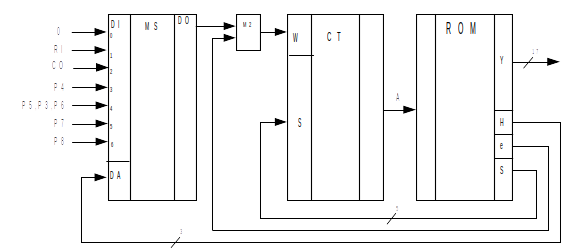
\includegraphics[width=0.8\linewidth]{images/course_ma_temp}
	\caption{УА с регулярной адресацией}
	\label{fig:courseschemema}
\end{figure}

На вход УА подаются сигналы от операционного автомата соответствующие логическим блокам алгоритма. С выхода управляющего автомата снимаются микроинструкции хранящиеся в ПЗУ (ROM) УА. Микроинструкции обеспечивают наличие необходимых управляющих сигналов на элементах операционного автомата в соответствии с выбранным блоком алгоритма. Также в ПЗУ содержится адресная часть позволяющая в следующем такте работы выбрать новый адрес управляющей памяти.

Мультиплексор обеспечивает выбор входного сигнала поступившего от ОА в соответствии с адресом хранящимся в ПЗУ.
Элемент М2 позволяет инвертировать значения входного сигнала что обеспечивает подстройку УА под конкретные схемотехнические решения.

Счётчик при поступлении на вход W нуля производит загрузку адреса микроинструкции на вход S', а при поступлении единицы осуществляет инкрементацию адреса, хранящегося в счётчике.



\if 0
В конкретной реализации на информационные входы мультиплексора подаются следующие сигналы:
\hypertarget{name}{}
\begin{itemize}
	\small
	\item Константа нуля;
	\item Ma\_IS\_NULL (признак нуля мантиссы А);
	\item Mb\_IS\_NULL (признак нуля мантиссы B);
	\item A<B (признак того, что порядок числа A меньше порядка числа B);
	\item A\_IS\_ANSWER (признак того, что ответ хранится в регистрах числа A);
	\item CT\_dP\_IS\_NULL (признак того, что счетчик разницы порядков хранит "ноль");
	\item CT\_Pa\_IS\_NULL (признак переполнения счетчика порядка числа A в большую сторону);
	\item CT\_Pa\_IS\_MAX  (признак переполнения счетчика порядка числа A в меньшую сторону);
	\item $\left|m\_a\pm m\_b\right|>1$ (признак того, что модуль алгебраической суммы операндов больше единицы);
	\item op\_normalized (признак нормализации операндов);
\end{itemize}

Укажем необходимые признаки, которые впоследствии будут вырабатываться управляющим автоматом. См. таблицу \ref{tab:signals5}.
\begin{table}[h!]
	\centering
	\small
	\begin{tabular}{|m{0.17\linewidth}|m{0.7\linewidth}|}
		\hline
		\textbf{Признак} & \textbf{Назначение} \\ \hline
		$S$ & Хранит адрес следующей операции \\ \hline
		$Н$ & Адресный вход мультиплексора \\ \hline
		$R0$ & Сигнализирует об окончании операции деления \\ \hline
		$overflow$ & Сигнализирует об ошибке обработки -- переполнение \\ \hline
		$L\_Ma$ & Загрузка в регистр $RG\_Ma$ \\ \hline
		$SHIFT\_Ma$ & Правый сдвиг регистра $RG\_Ma$ если $SHIFT\_Ma\_Left=0$ и левый, если  $SHIFT\_Ma\_Left=1$ \\ \hline
		$RST$ & Асинхронный сброс всех элементов \\ \hline
		$COUNT\_Pa$ & Счет. Декремент счетчика, если $L\_CT_\_Pa==1$ \\ \hline
		$L\_CT\_Pa$ & Загрузка счетчика $CT\_Pa$ \\ \hline
		$CHANGE$ & Выбор источника загрузки в регистры мантисс и порядка чисел A и B \\ \hline
		$e$ & Управляющий сигнал для счетчика. Если $e=1$, следует выполнить загрузку, а если $e=0$ -- инкрементировать счетчик. \\ \hline
	\end{tabular}
	\caption{Осведомительные сигналы (признаки)}
	\label{tab:signals5}
\end{table}

\fi







\section{Заполнение памяти}

\subsection{Деление двух целых чисел в дополнительном коде}

Приведем таблицу переходов для управляющего автомата выполненного по схеме с регулярной адресацией для операции нахождения частного двух чисел в дополнительном коде. См. таблицу \ref{tab:coursedivsteps}.

\begin{table}[h!]
	\centering
	\begin{tabular}{|r||l|l|l|l|}
		\hline
		\multicolumn{1}{|l||}{\textbf{A}} & \textbf{Y} & \textbf{H} & \textbf{S} & \textbf{e} \\ \hline
		0 & m0 & 0 & 1 & 1 \\ \hline
		1 & m1 & 0 & 4 & 1 \\ \hline
		2 & m01 & 0 & 2 & x \\ \hline
		3 & m2 & 2 & 0 & 0 \\ \hline
		4 & m3 & 0 & 4 & 0 \\ \hline
		5 & m02 & 3 & 3 & x \\ \hline
		6 & m6 & 0 & 0 & 0 \\ \hline
		7 & m5 & 0 & 3 & 0 \\ \hline
		8 & m4 & 2 & 2 & x \\ \hline
		9 & m03 & 1 & 1 & x \\ \hline
	\end{tabular}
	\caption{Деление чисел в доп. коде. Таблица переходов}
	\label{tab:coursedivsteps}

\end{table}

Также приведем таблицу заполнения памяти ПЗУ управляющего автомата. См. таблицу \ref{tab:coursesummemory} в \hyperref[tam]{Приложении А}.

\subsection{Сложение чисел в экспоненциальном формате}

	Приведем таблицу переходов для управляющего автомата выполненного по схеме с регулярной адресацией для операции нахождения суммы двух чисел в экспоненциальной форме. См. таблицу \ref{tab:coursesumsteps}.
	%\newpage
\begin{longtable}{|m{0.1\linewidth}||m{0.1\linewidth}|m{0.1\linewidth}|m{0.1\linewidth}|m{0.1\linewidth}|}
	
	\hline	
	\multicolumn{1}{|l||}{\textbf{A}} & \textbf{Y} & \multicolumn{1}{l|}{\textbf{H}} & \multicolumn{1}{l|}{\textbf{S}} & \multicolumn{1}{l|}{\textbf{e}} \\ \hline
	\endfirsthead
	
	\multicolumn{5}{c}%
	{{\bfseries \tablename\ \thetable{} -- продолжение}} \\
	
	\hline	
	\multicolumn{1}{|l||}{\textbf{A}} & \textbf{Y} & \multicolumn{1}{l|}{\textbf{H}} & \multicolumn{1}{l|}{\textbf{S}} & \multicolumn{1}{l|}{\textbf{e}} \\ \hline
	\endhead
	
	\hline \multicolumn{5}{c}{{См. след. страницу}} %\\ \hline
	\endfoot
	
	%\hline \hline
	\endlastfoot

		0 & m1 & \multicolumn{1}{l|}{x} & 1 & \multicolumn{1}{l|}{x} \\ \hline
		1 & m2 & 2 & 15 & 0 \\ \hline
		2 & m01 & 1 & 16 & 0 \\ \hline
		3 & m02 & 3 & 5 & 1 \\ \hline
		4 & m6 & \multicolumn{1}{l|}{x} & 5 & \multicolumn{1}{l|}{x} \\ \hline
		5 & m03 & 5 & 9 & 0 \\ \hline
		6 & m04 & 4 & 18 & 0 \\ \hline
		7 & m8 & 0 & 19 & 1 \\ \hline
		8 & m9 & 5 & 19 & 1 \\ \hline
		9 & m10 & 8 & 11 & 1 \\ \hline
		10 & m11 & 6 & 13 & 0 \\ \hline
		11 & m05 & 9 & 14 & 0 \\ \hline
		12 & m12 & 7 & 11 & 1 \\ \hline
		13 & m13 & 0 & 0 & 1 \\ \hline
		14 & m14 & 0 & 0 & 1 \\ \hline
		15 & m3 & 0 & 0 & 1 \\ \hline
		16 & m4 & \multicolumn{1}{l|}{x} & 17 & \multicolumn{1}{l|}{x} \\ \hline
		17 & m5 & 0 & 0 & 1 \\ \hline
		18 & m7 & 0 & 0 & 1 \\ \hline
		19 & m15 & 0 & 8 & 1 \\ \hline
	\caption{Сложение чисел в экспоненциальной форме. Таблица переходов}
	\label{tab:coursesumsteps}
\end{longtable}

Также приведем таблицу заполнения памяти ПЗУ управляющего автомата. См. таблицу \ref{tab:coursesummemory} в \hyperref[tam]{Приложении А}.

\section{Заключение}
В ходе данной курсовой работы был рассмотрен алгоритм деления двух целых чисел без восстановления остатка дополнительном коде и алгоритм нахождения суммы двух чисел, представленных в формате с одинарной точностью. 

Рассмотренные алгоритмы изучены и реализованы на спроектированном вычислительном устройстве --- синхронном конечном автомате, управляющий автомат которого выполнен по схеме с регулярной адресацией.

Освоенные в течение курса теоретические положения были применены на практике, что позволило использовать аппарат теории автоматов для решения реальных задач проектирования дискретных устройств с памятью. 

В ходе выполнения курсовой работы были приобретены необходимые навыки и умения в проектировании операционных блоков вычислительных устройств.


\newpage{
	\centering
	\anonsection{БИБЛИОГРАФИЧЕСКИЙ СПИСОК}
}
\label{biblio}
\begin{enumerate}
	\item Антик М.И. Теория автоматов в проектировании цифровых схем
	[Электронный ресурс]: Учебное пособие / Антик М.И., Казанцева
	Л.В. — М.: МИРЭА – Российский технологический университет,
	2020.
	\item Антик М.И., Синхронные цифровые автоматы [Электронный ресурс]:
	монография / М.И. Антик, А.М. Романов. — М.: МГТУ МИРЭА,
	2014. — Электрон. опт. диск (ISO), НТБ МИРЭА А72
	\item Антик М.И., Триггеры [Электронный ресурс]: учебное пособие для
	студентов, обучающихся по направлениям подготовки 230100 и спец.
	230101 "Вычислительные машины, системы, комплексы и сети" /
	М.И. Антик, А.М. Романов. — М.: МГТУ МИРЭА, 2012. — Электрон.
	опт. диск (ISO), НТБ МИРЭА А72
	\item Зайцев Е.И., Прикладная теория цифровых автоматов: учебное пособие / Е.И. Зайцев, В. В. Макаров. — М.: МИРЭА, 2018. — 112 с. —
	Библиогр.: с. 111 (7 назв.), НТБ МИРЭА З-17
	\item Горбатов В.А. Теория автоматов: учеб. для студентов втузов – М.:
	АСТ: Астрель. 2008. – 559 с.
	\item  Карпов Ю.Г. Теория автоматов /– СПб: Питер. 2003. – 208 с.
\end{enumerate}

\newpage{
	\centering
	\anonsection{ПРИЛОЖЕНИЕ А}
}
\label{tam}

\begin{figure}[h!]
	\centering
	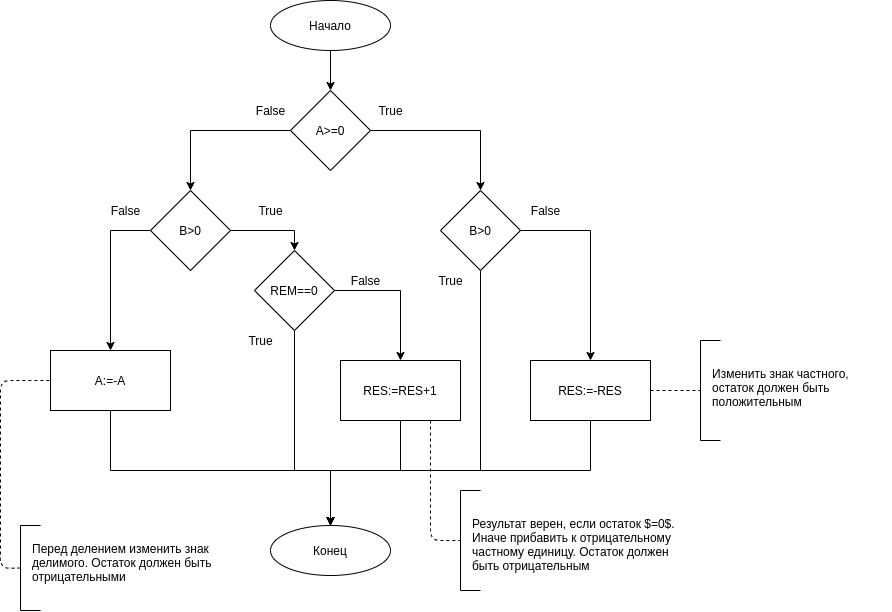
\includegraphics[width=0.7\linewidth]{divide_algorithm_course_correction}
	\caption {Алгоритм коррекции результата}
	\label{img:algorithmcorrection}
\end{figure}


%\newpage
\begin{figure}[h!]
	\centering
	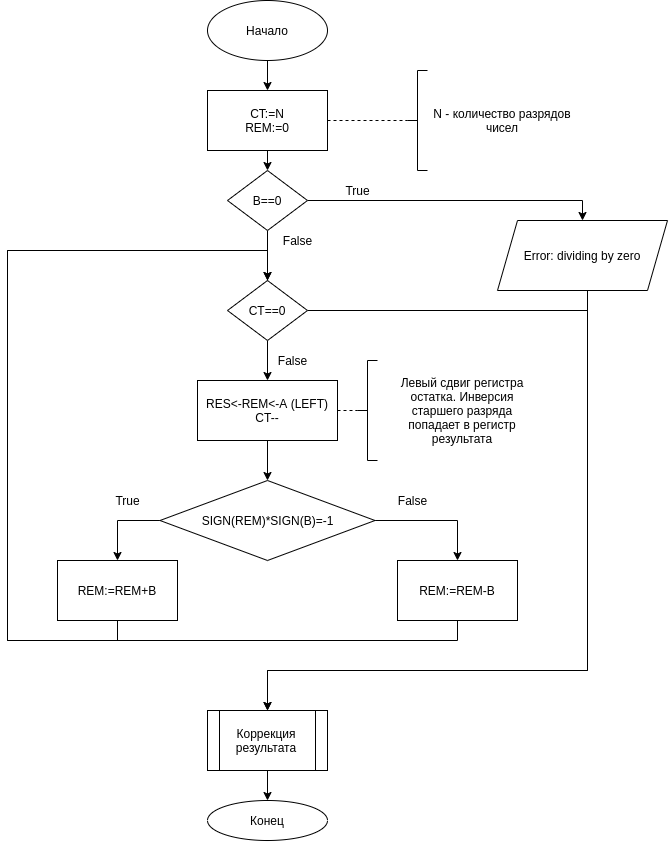
\includegraphics[width=0.6\linewidth]{divide_algorithm_course}
	\caption {Алгоритм деления чисел}
	\label{img:algorithmcourse}
\end{figure}
\newpage
\begin{figure}[h!]
	\centering
	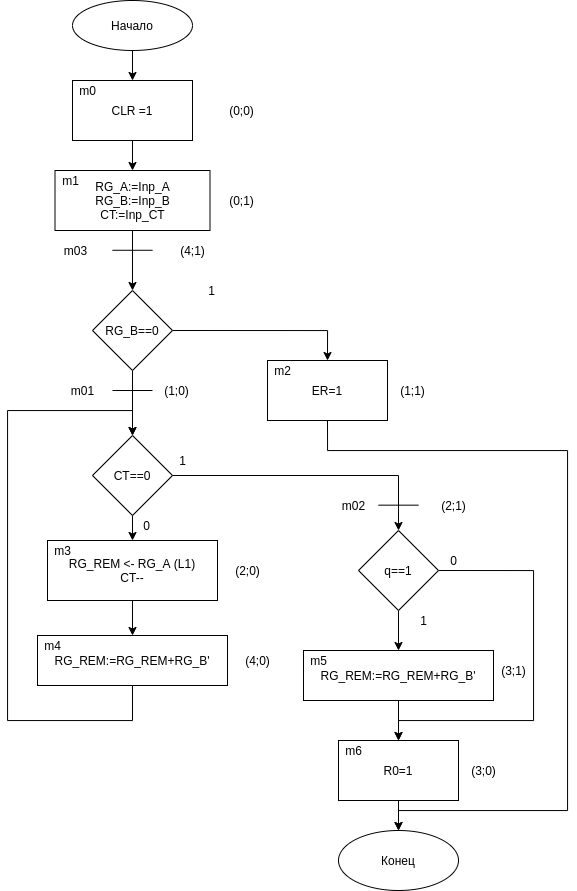
\includegraphics[width=0.7\linewidth]{images/course_algorithm_divide_machine}
	\caption{Деление двух чисел. Блок-схема работы автомата}
	\label{fig:coursealgorithmdividemachine}
\end{figure}
\newpage
\begin{figure}[h!]
	\centering
	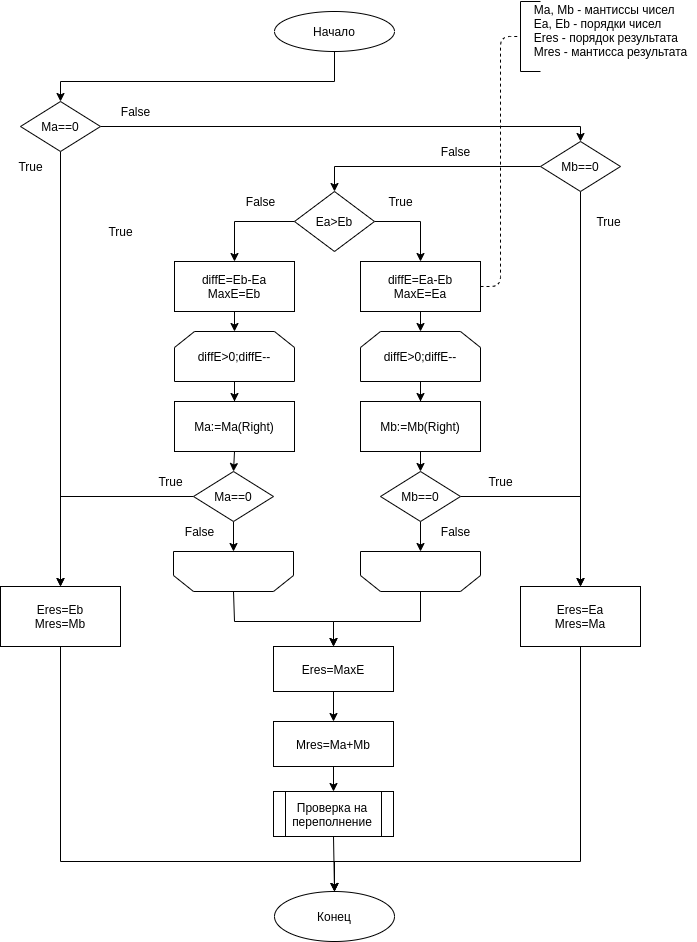
\includegraphics[width=0.7\linewidth]{images/course_algorithm_sum}
	\caption{Алгоритм суммирования чисел в доп. коде}
	\label{fig:coursealgorithmsum}
\end{figure}

\newpage
\begin{figure}[h!]
	\centering
	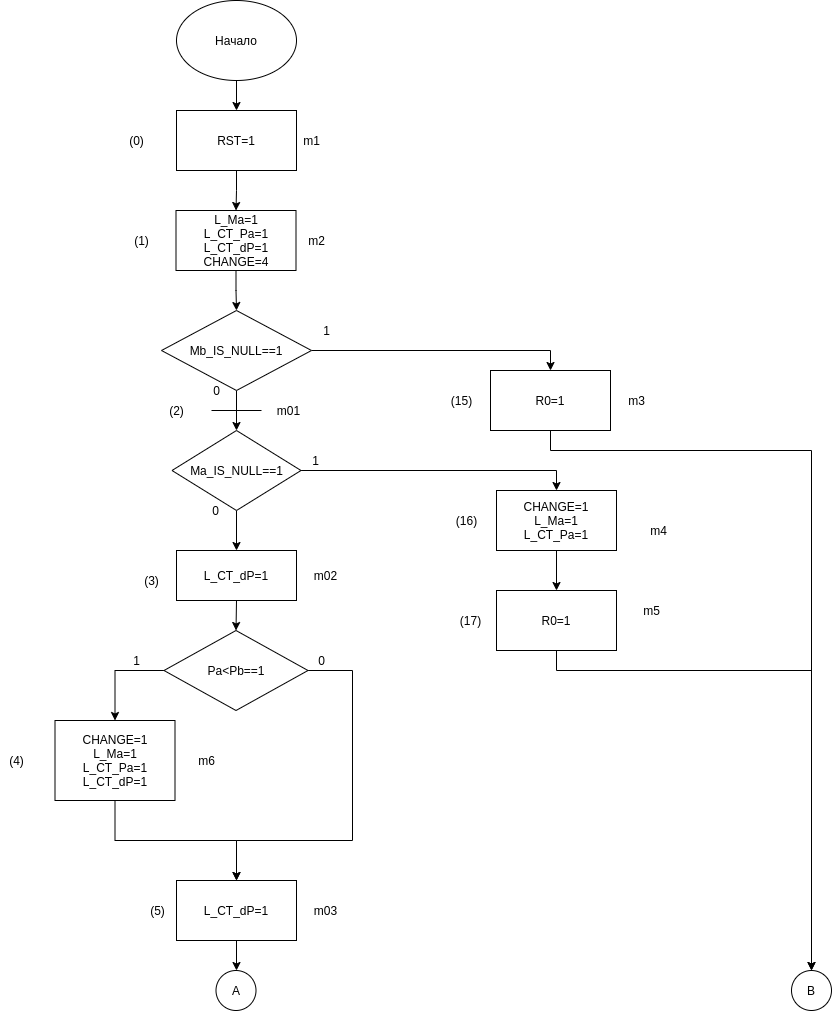
\includegraphics[width=0.44\linewidth]{algorithm5.1}
	%\caption {Алгоритм сложения чисел с плавающей точкой. Часть 1}
	\label{fig:coursealgorithmmachine1}
\end{figure}
%\newpage
\begin{figure}[h!]
	\centering
	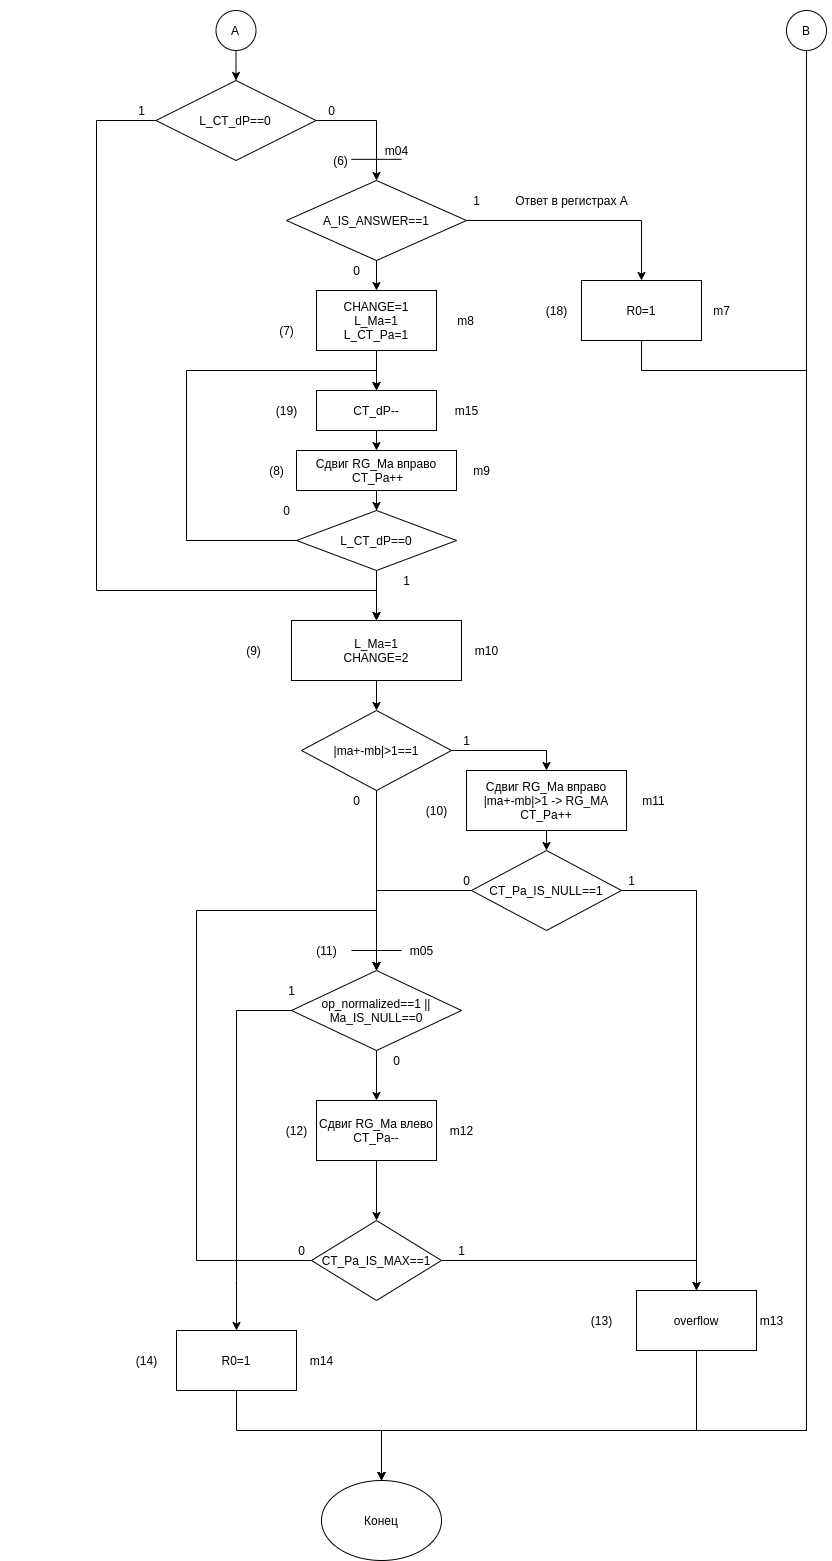
\includegraphics[width=0.46\linewidth]{algorithm5.2}
	\caption {Алгоритм сложения чисел. Блок-схема работы автомата}
	\label{fig:coursealgorithmmachine2}
\end{figure}
\newpage
% TODO: \usepackage{graphicx} required
\begin{figure}[h!]
	\centering
	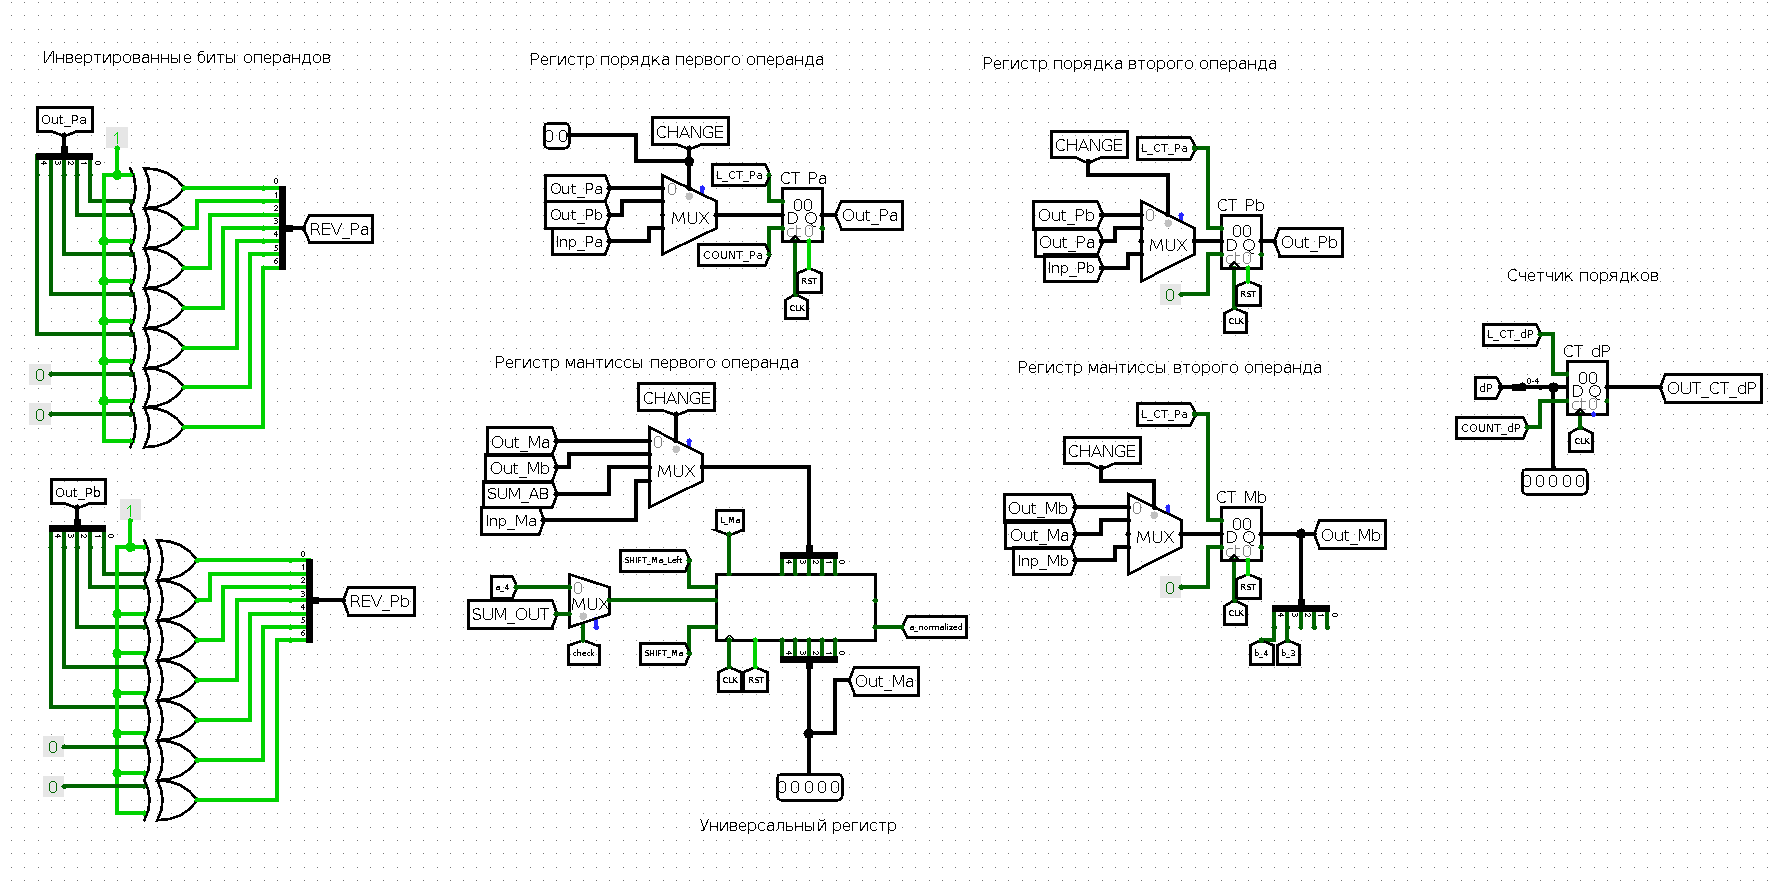
\includegraphics[width=\linewidth]{images/course_operation_automat2}
	\caption{Сложение чисел. Операционный автомат}
	\label{fig:courseoperationautomat2}
\end{figure}

\newpage
\begin{landscape}
\begin{table}[h!]
%	\small
	\centering
	\begin{tabular}{|r||l|r|l|l|l|l|l|l|l|l|l|l|l|}
		\hline
		\multicolumn{1}{|l||}{\textbf{A}} & \textbf{N} & \multicolumn{1}{l|}{\textbf{e}} & \textbf{L\_RG\_A} & \textbf{L\_B} & \textbf{L\_REM} & \textbf{SHIFT} & \textbf{CT} & \textbf{L\_CT} & \textbf{CLR} & \textbf{ER} & \textbf{R0} & \textbf{H} & \textbf{S} \\ \hline \hline
		0 & m0 & 1 & 0 & 0 & 0 & 0 & 0 & 0 & 1 & 0 & 0 & 00 & 001 \\ \hline
		1 & m1 & 1 & 1 & 1 & 1 & 0 & 0 & 1 & 0 & 0 & 0 & 00 & 100 \\ \hline
		2 & m01 & \multicolumn{1}{l|}{x} & 0 & 0 & 0 & 0 & 0 & 0 & 0 & 0 & 0 & 10 & 010 \\ \hline
		3 & m2 & 0 & 0 & 0 & 0 & 0 & 0 & 0 & 0 & 1 & 0 & 00 & 000 \\ \hline
		4 & m3 & 0 & 0 & 0 & 0 & 1 & 1 & 1 & 0 & 0 & 0 & 11 & 100 \\ \hline
		5 & m02 & \multicolumn{1}{l|}{x} & 0 & 0 & 0 & 0 & 0 & 0 & 0 & 0 & 0 & 00 & 011 \\ \hline
		6 & m6 & 0 & 0 & 0 & 0 & 0 & 0 & 0 & 0 & 0 & 1 & 00 & 000 \\ \hline
		7 & m5 & 0 & 0 & 0 & 1 & 0 & 0 & 0 & 0 & 0 & 0 & 00 & 011 \\ \hline
		8 & m4 & \multicolumn{1}{l|}{x} & 0 & 0 & 1 & 0 & 0 & 0 & 0 & 0 & 0 & 10 & 010 \\ \hline
		9 & m03 & \multicolumn{1}{l|}{x} & 0 & 0 & 0 & 0 & 0 & 0 & 0 & 0 & 0 & 01 & 001 \\ \hline
	\end{tabular}
\caption{Деление чисел в доп. коде. Таблица заполнения памяти}
\label{tab:coursedivmemory}
\end{table}
\end{landscape}

\newpage
\begin{landscape}

\begin{table}[htbp]
	\small
	\begin{tabular}{|c||c|c|c|c|c|c|c|c|c|c|c|c|c|c|c|}
		\hline
		\textbf{A} & \textbf{N} & \textbf{S} & \textbf{R0} & \textbf{RST} & \textbf{L\_ma} & \textbf{SFT\_Ma} & \textbf{SFT\_Ma\_L} & \textbf{L\_CT\_Pa} & \textbf{COUNT\_Pa} & \textbf{CHANGE} & \textbf{L\_CT\_dP} & \textbf{COUNT\_dP} & \textbf{m\_n} & \textbf{H} & \textbf{e} \\ \hline \hline
		0 & m1 & 1 & 0 & 1 & 0 & 0 & 0 & 0 & 0 & 00 & 0 & 0 & 0 & 0 & 0 \\ \hline
		1 & m2 & 15 & 0 & 0 & 1 & 0 & 0 & 1 & 0 & 11 & 1 & 0 & 0 & 2 & 0 \\ \hline
		2 & m01 & 16 & 0 & 0 & 0 & 0 & 0 & 0 & 0 & 00 & 0 & 0 & 0 & 1 & 0 \\ \hline
		3 & m02 & 5 & 0 & 0 & 0 & 0 & 0 & 0 & 0 & 00 & 1 & 0 & 0 & 3 & 1 \\ \hline
		4 & m6 & 5 & 0 & 0 & 1 & 0 & 0 & 1 & 0 & 01 & 1 & 0 & 0 & 0 & 0 \\ \hline
		5 & m03 & 9 & 0 & 0 & 0 & 0 & 0 & 0 & 0 & 00 & 1 & 0 & 0 & 5 & 0 \\ \hline
		6 & m04 & 18 & 0 & 0 & 0 & 0 & 0 & 0 & 0 & 00 & 0 & 0 & 0 & 4 & 0 \\ \hline
		7 & m8 & 19 & 0 & 0 & 1 & 0 & 0 & 1 & 0 & 01 & 0 & 0 & 0 & 0 & 1 \\ \hline
		8 & m9 & 19 & 0 & 0 & 0 & 1 & 0 & 0 & 1 & 00 & 0 & 0 & 0 & 5 & 1 \\ \hline
		9 & m10 & 11 & 0 & 0 & 1 & 0 & 0 & 0 & 0 & 10 & 0 & 0 & 0 & 8 & 1 \\ \hline
		10 & m11 & 13 & 0 & 0 & 0 & 1 & 0 & 0 & 1 & 00 & 0 & 0 & 0 & 6 & 0 \\ \hline
		11 & m05 & 14 & 0 & 0 & 0 & 0 & 0 & 0 & 0 & 00 & 0 & 0 & 0 & 9 & 0 \\ \hline
		12 & m12 & 11 & 0 & 0 & 0 & 1 & 1 & 1 & 1 & 00 & 0 & 0 & 0 & 7 & 1 \\ \hline
		13 & m13 & 0 & 0 & 0 & 0 & 0 & 0 & 0 & 0 & 00 & 0 & 0 & 1 & 0 & 1 \\ \hline
		14 & m14 & 0 & 1 & 0 & 0 & 0 & 0 & 0 & 0 & 00 & 0 & 0 & 0 & 0 & 1 \\ \hline
		15 & m3 & 0 & 1 & 0 & 0 & 0 & 0 & 0 & 0 & 00 & 0 & 0 & 0 & 0 & 1 \\ \hline
		16 & m4 & 17 & 0 & 0 & 1 & 0 & 0 & 1 & 0 & 01 & 0 & 0 & 0 & 0 & 0 \\ \hline
		17 & m5 & 0 & 1 & 0 & 0 & 0 & 0 & 0 & 0 & 00 & 0 & 0 & 0 & 0 & 1 \\ \hline
		18 & m7 & 0 & 1 & 0 & 0 & 0 & 0 & 0 & 0 & 00 & 0 & 0 & 0 & 0 & 1 \\ \hline
		19 & m15 & 8 & 0 & 0 & 0 & 0 & 0 & 0 & 0 & 00 & 1 & 1 & 0 & 0 & 1 \\ \hline
	\end{tabular}
	\caption{Сложение чисел в экспоненциальной форме. Таблица заполнения памяти}
	\label{tab:coursesummemory}
\end{table}
\end{landscape}
\end{document}


